% \documentclass[a4paper]{article}
\documentclass[]{report}

\usepackage{tgtermes}         % for the looks
\usepackage[T1]{fontenc}     % to hypenate accented characters correctly
\usepackage[utf8]{inputenc}  % just in case we go for non-ascii
\usepackage{tikz}            % the graphics
\usepackage{textcomp}        % for \textregistered
\usepackage{anyfontsize}
\usepackage{hyperref}
\usepackage{titlesec}        % adjusting document class formatting
\usepackage{titletoc}        % adjusting document /tableofcontents
\usepackage{multicol}
\usepackage{changepage}
\usepackage[margin=1.5in]{geometry} % 1.75" is default

\definecolor{myColor}{RGB}{101,28,34} % Cover/accent color 

% \titleformat{\chapter}[block]
%   {\normalfont\huge\bfseries}{\thechapter.}{1em}{\Huge}

\titlespacing*{\chapter}{0pt}{-19pt}{0pt}

\dottedcontents{chapter}[4.5em]{\bfseries\normalsize\vspace{.75em}}{3.2em}{1pc} % \tableofcontents


\renewcommand{\thechapter}{\Roman{chapter}} % Forces roman numerals 

\titleformat{\chapter}[display]
      {\bfseries\Large}
      % {\filleft\MakeUppercase{xxx\chaptertitlename} ttt\Huge\thechapter}
      {\filleft\Huge\thechapter}
      {0ex}
      {\color{myColor}\titlerule[3pt]\color{black}
      \vspace{1ex}%
      \filright}
      [\vspace{.5ex}%
      \color{myColor}{\titlerule[3pt]}]



%%%%%%%%%%%%%%%%%%%%%%%%%%%%%%%%%%%%%%%

% \newcommand{\meal}[5]{
% \chapter{\uppercase{#1}}  % recipe name
% \vspace{0.5cm}
% \textit{#2}\vspace{0.5cm} \\                      % description (if needed)
% {\textbf{Serves: #3}}                % serving size
% \vspace{0.5cm}\\
% \begin{minipage}[t]{0.5\textwidth}
%       #4                            % list of ingredients 
% \end{minipage}
% \begin{minipage}[t]{0.5\textwidth}
%       \vspace{-0.7cm}
%       \textbf{#5}                            % cooking instructions
% \end{minipage}
% }

\newcommand{\meal}[5]{
\chapter{\uppercase{#1}}  % recipe name
\vspace{0.5cm}
\textit{#2}\vspace{0.5cm} \\                      % description (if needed)
{\textbf{Serves: #3}}                % serving size
\vspace{0.1cm}\\
\begin{adjustwidth}{-1.7em}{1.5em}
\begin{minipage}[t]{0.45\textwidth}
      #4                            % list of ingredients 
\end{minipage}
\begin{minipage}[t]{0.59\textwidth}
      \vspace{-0.7cm}
      \textbf{#5}                            % cooking instructions
\end{minipage}
\end{adjustwidth}
}

% \newcommand{\meal}[5]{
% \chapter{\uppercase{#1}}  % recipe name
% \vspace{0.5cm}
% \textit{#2}\vspace{0.5cm} \\                      % description (if needed)
% {\textbf{Serves: #3}}                % serving size
% \vspace{1cm}\\
% \begin{multicols}{2}
%       #4                            % list of ingredients 
% \end{multicols}
% \textbf{#5}
% }


%%%%%%%%%%%%%%%%%%%%%%%%%%%%%%%%%%%%%%%








\begin{document}

\thispagestyle{empty}

%%%%%%%%%%%%%%%%%%%%% Cover Page %%%%%%%%%%%%%%%%%%%%%

\begin{tikzpicture}[remember picture,overlay]

\node [align=center] at (current page.north) % upper
      {\begin{tikzpicture}[remember picture, overlay]
	  \fill[myColor] (-10,0) rectangle (10,-0.5);
	  \node[anchor=north] at (0,-0.5) {\fontsize{29}{34}\selectfont\textit{Recipes I want to keep track of}};
      \end{tikzpicture}};
      


\node [yshift=5cm] at (current page.center) % title
      {\begin{tikzpicture}[remember picture, overlay]
          \fill[myColor] (-9.5,-5) rectangle (9.5 ,1);
          \node[align=center] at (0,-2)
               {\resizebox{1.57\linewidth}{!}{\hspace{.25cm}\Huge\color{white}Food\hspace{2.1cm}}};
	       \node[anchor=east,align=right] at (1.2,-5.5) {\fontsize{29}{34}\selectfont\color{black}\textit{In no particular order}};
      \end{tikzpicture}};

\node [align=center, yshift=-6cm] at (current page.center) % animal image
      {\begin{tikzpicture}[remember picture, overlay]
          \node[anchor=center,align=center] at (0,5)
               {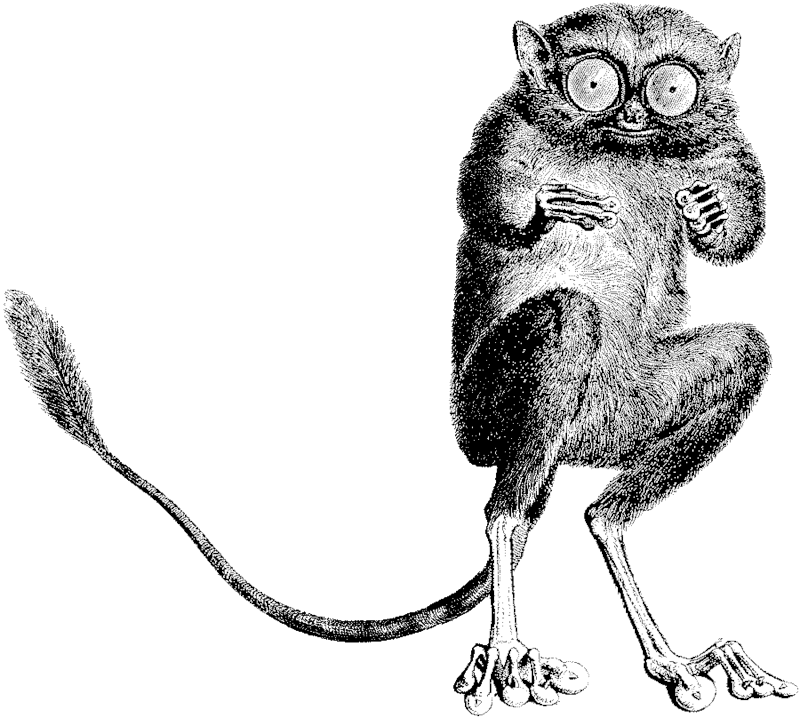
\includegraphics[width=1.65\textwidth]{tarsier3.png}};
      \end{tikzpicture}};

% \node [shift={(-5cm,-5cm)}] at (current page.north east) % Revision 2
%       {\begin{tikzpicture}[remember picture, overlay]
%           \draw[fill=black] (0,5) -- (1.5,5) -- (5,1.5) -- (5,0) -- cycle ;
%           \node[inner sep=0pt,rotate=-45] (rev) at (2.9,2.9) {\huge\color{white}\textbf{Revision 2}};
%       \end{tikzpicture}};

\node [align=center] at (current page.south) % bottom
      {\begin{tikzpicture}[remember picture, overlay]
          \node[anchor=south west, align=left] at (-10,0.5)
               {\resizebox{.3\linewidth}{!}
                 {\Huge\color{black}\fontfamily{phv}\selectfont
                   {O\color{myColor}'\color{black}RLY\textsuperscript{\color{myColor}\Large\textbf{?}}}}};
               \node[anchor=south east, align=right] at (10,0.5) {\Huge\color{black}\textit{Patrick McMackin}};
      \end{tikzpicture}};

\end{tikzpicture}

%%%%%%%%%%%%%%%%%%%%% Cover Page %%%%%%%%%%%%%%%%%%%%%


\tableofcontents

%%%%%%%%%%%%%%%%%%%%%%%%%%%%%%%%%%%%%%%%
      % \meal{RecipeTitle}
      %       {OptionalComment}
      %       {5--8}                % Serving Size
      %       {\begin{itemize}      % Ingredients
      %             \item 
      %       \end{itemize}}
      %       {\begin{enumerate}    % Cooking Instructions
      %             \item  
      %       \end{enumerate}}
%%%%%%%%%%%%%%%%%%%%%%%%%%%%%%%%%%%%%%%%


      \meal{Spicy-Sweet Sambal Pork Noodles}
            {From Bon Appetit}
            {6--8}
            {\begin{itemize}
                  \item 4 Tbsp. extra-virgin olive oil
                  \item 4 lb. ground pork, divided
                  \item 2" piece fresh ginger, peeled, finely chopped
                  \item 12 Garlic cloves, minced
                  \item 4 Tbsp. Sugar
                  \item 4 Tbsp. Tomato paste
                  \item 4 Sprigs basil, plus garnish
                  \item 2 Cup hot chili paste (such as sambal oelek)
                  \item 2 Cup soy sauce
                  \item 2 Cup unseasoned rice vinegar
                  \item 2 lbs ramen noodles
                  \item Salt/Pepper
                  \item 4 Tbsp. unsalted butter
                  \item 2-3 Broccoli crowns
            \end{itemize}}
            {\begin{enumerate}
                  \item  Heat oil in a large wide heavy pot over medium-high. Add half of pork, breaking apart with wooden spoon. Cook until well browned underneath, about 5 mins. Turn and continue to cook until pork is browned on 2--3 sides, about 5 mins.
                  \item Add ginger, garlic, sugar, and remaining pork and cook until meat is nearly cooked through, about 5 mins. Add tomato paste and 2 basil sprigs. Cook, stirring  occasionally, until paste darkens, about 2 minutes.
                  \item Add chili paste, soy sauce, vinegar, and 2 cups water. Bring to a simmer, reduce heat to low, and cook, uncovered and stirring occasionally, until sauce is slightly thickened and flavors have melded, 30—45 minutes.
                  \item Dice broccoli finely, add to pot in last about 10 minutes of cooking
                  \item Cook noodles in a large pot of boiling salted water, until 1 minute short of al dente. Add to sauce with butter and a splash of pasta cooking liquid. Simmer, toss, until sauce begins to cling to noodles, about 1 minute. Add basil.
            \end{enumerate}}    


      \meal{Halal Chicken and rice}
            {From Ethan Chlebowski, optionally add red sauce (or make chicken spicy). Season aggressivly and sear the chicken hard. }
            {6--8}                % Serving Size
            {\begin{itemize}      % Ingredients
                  \item 4 lbs skinless Chicken thighs
                  \item Salt/Pepper
                  \item Cayenne
                  \item 5 whole cloves, crushed
                  \item Cumin
                  \item Oregano
                  \item 3 Garlic cloves
                  \item Lemon juice
                  \item Mayo
                  \item 2 Tbsp Butter 
                  \item 1/2 Onion, diced
                  \item Turmeric 
                  \item Smoked Paprika 
                  \item 1 Bay leaf
                  \item 2 cups Basmati rice
                  \item 2 cups water or stock 
                  \item plain Greek yogurt
                  \item 10 g white Vinegar
            \end{itemize}}
            {\begin{enumerate}    % Cooking Instructions
                  \item Marinated Chicken: Salt the chicken thighs and set them aside. Crush the cloves and cumin in a mortar and pestle. Add oregano, black pepper, cayenne, and garlic cloves into the mortar with the spices and crush into a rough paste. In a large mixing bowl, combine the lemon juice, mayo, and spice mixture. Add the chicken thighs and thoroughly coat the exterior. Cover and place in the fridge for up to 24hrs or cook right away.
                  \item Place a pan over high to medium-high heat. Once hot, sear the chicken thighs until deeply browned. Chop the chicken into pieces in the pan
                  \item Yellow Rice: Melt butter in a pot over medium heat. Add onion, cumin, turmeric, smoked paprika, pepper, and bay leaf. Stir aromatics together until fragrant but not burnt, about 30 seconds. Add the rice to the pan with the aromatics and mix. Lightly toast the rice and stir for about 2 minutes. Add chicken broth, turn up the heat, and cover the pan to bring to a boil. Turn the heat to the lowest setting. Let rice steam covered for about 20 mins
                  \item Mix white sauce (2 parts mayo, 1 part yogurt, oregano, lemon juice, vinegar, salt, paprika, MSG, garlic powder) in bowl to taste, drizzel over chicken and rice. Serve with simple lettuce/tomato/onion salad and naan
            \end{enumerate}}

      \meal{Basic Chicken Curry}
            {Optionally add MSG, lemon grass, curry powder, ect}
            {5--8}
            {\begin{itemize}
                  \item 3 cups (dry) rice (cooked)
                  \item 4lbs chicken thighs
                  \item Cinnamon
                  \item Tumeric
                  \item Garam Masala
                  \item 1 Hot chili (diced)
                  \item 2 Bell peppers (diced)
                  \item 2 Large onion (diced)
                  \item Large knob ginger (ground to paste)
                  \item 5--6 Cloves garlic (ground to paste)
                  \item Ground cardamom
                  \item Chili powder
                  \item Cayenne powder
                  \item Diced/crushed tomatoes (2x 28 oz cans)
                  \item 1--2 Cups stock
                  \item Coconut milk (2-3 140z cans)
                  \item Bay leaves
                  \item Dice coriander
                  \item Salt/pepper
            \end{itemize}}
            {\begin{enumerate}
                  \item Marinade chicken with oil, salt, 1 tbs tumeric, 1 tbs garam masala, 1/4 tps cinnamon
                  \item Brown chicken in batches. (No need to cook all the way)
                  \item Remove chicken, add chili, peppers, onion, garlic, ginger. Cook
                  \item Add 1/4 tps ground cardamom, 1 ths garam masala, 1 tbs chili powder, cayenne powder, salt, pepper and bay leaves. Bloom spices. (Add spices generously, and "by the heart")
                  \item Return chicken to pot, add tomatos, stock
                  \item Simmer about 30 minutes without lid
                  \item Add coconut milk, cook another 15--20 mins
                  \item Mix in diced coriander, serve over rice
            \end{enumerate}}






      \meal{Slow cooker chicken tacos}
            {Dead easy}
            {6--8}
            {\begin{itemize}
                  \item Chicken breast (4--5 lbs)
                  \item Black beans drained (28oz can)
                  \item Corn drained (14oz can)
                  \item Taco seasoning package
                  \item Ranch seasoning package
                  \item Adobo peppers (2-3)
                  \item Crushed/diced tomatoes (28oz can)
                  \item Cream cheese (3/4 package)
                  \item Cilantro
                  \item Salt/Pepper + whatever spices (Cumin...)
            \end{itemize}}
            {\begin{enumerate}
                  \item Slowcook 3 hours on high
                  \item Remove and shred chicken
                  \item Return chicken, add chopped cilantro
                  \item Serve on wraps or with rice
            \end{enumerate}}


      \meal{Beef Chili}
            {From J Kenji Lopez Alt}
            {6--8}
            {\begin{itemize}
                  \item 3lbs Ground beef
                  \item 2 Onions
                  \item 6ish Cloves garlic
                  \item 6ish Anchovy fillets
                  \item 1 small can of Peppers in adobo
                  \item 1 tbps Oregano
                  \item 1tbps Cumin
                  \item 1/2 cup Tomato paste
                  \item 1 28oz can Tomato (whole or chunk)
                  \item 1 28oz can Black beans (or kidney)
                  \item 2ish cups Frozen corn
                  \item 1-2 cups Chicken stock
                  \item 3 thps Instant cornmeal (maseca)
                  \item 1 tbps Cocoa powder
                  \item MSG
                  \item Worcestershire sauce
                  \item Soy Sauce
                  \item 1 tbps Brandy
                  \item 3 tbps Hot sauce
                  \item Salt/Pepper
            \end{itemize}}
            {\begin{enumerate}
                  \item Brown beef with oil fairly hard (in batches). Add diced onions to the end to soften, add garlic in last 60 seconds of cooking
                  \item Mash anchovy fillets with fork, dice peppers and add all ingredients to slowcooker on low for 8 hours (include adobo sauce). Salt/pepper
                  \item Serve with garnishes (greens, cheese, sour cream, cornbread ect)
            \end{enumerate}}




        




      \meal{Enchiladas Verde con pollo}
            {From Adam Raguesa}
            {5--7}
            {\begin{itemize}
                  \item 4 lbs chicken thighs (skinless)
                  \item 2 large White onions
                  \item White wine
                  \item Cumin
                  \item Coriander
                  \item Paprika
                  \item Salt/Pepper
                  \item 4--8 Jalpe\~nos
                  \item 2 Limes
                  \item 4--5 Garlic cloves
                  \item Cilantro
                  \item 8oz Monterey Jack cheese
                  \item 16-20 7" Tortillas
            \end{itemize}}
            {\begin{enumerate}
                  \item  Fry the chicken thighs in olive oil until browned, and remove.
                  \item Roughly chop one of the onions and fry it in the same pot until golden. Put in maybe a teaspoon (or more) each of the ground cumin,               coriander and paprika, grind in some pepper, and fry the spices for a minute. Put the chicken back in, and cover with about half white wine, half water. Salt. Cover, reduce heat to a simmer, and cook until the chicken begins falling about (30 mins).
                  \item For the salsa verde, cut the chiles in half, scrape out and discard the seeds. Husk the tomatillos, rinse, and cut them in half. Roughly cut other onion. Put the veggies and lime into a wide pan and toss them in olive oil. Put the pan into the oven at 450 F. After the salsa has a bit of color, put in the whole peeled garlic cloves and stir. Cook maybe 20 mins total. Broil for a few minutes on high, Squeeze the lime juice and discard. Puree until smooth.
                  \item Grate up the cheese. Put maybe half a cup of the salsa into the chicken, along with half of the cheese. Mix up the filling and check for seasoning.
                  \item Grease a 7x11 inch baking dish. Dunk a tortilla into the salsa, scoop in a modest line of filling, and roll up the tortilla, seam-side down. Repeat until you've filled your baking dish and/or exhausted your filling. Spoon the extra salsa and cheese on top of the enchiladas. Bake uncovered until the cheese is browned, maybe 20 mins. Garnish with cilantro.
            \end{enumerate}}


      \meal{Orange peanut chicken bake}
            {Personal Favorite, found on Reddit}
            {5}
            {\begin{itemize}
                  \item 10 bone in, skin on Chicken thighs
                  \item 5-10 Chilis (anything hot)
                  \item 1 large Naval orange
                  \item 3/4 cup natural Peanut butter
                  \item 1 cup roasted Peanuts
                  \item Cilantro
                  \item 1/2 cup Soy sauce
                  \item 1/3 cup Fish sauce
                  \item 2-3 tbs Apple cider vinegar
                  \item 1/3 cup Brown sugar
                  \item 1 tbs Cumin
                  \item MSG
                  \item 2" knob Ginger
                  \item 5--7 cloves Garlic
                  \item White rice
                  \item Side veggie (Roast asparagus)
            \end{itemize}}
            {\begin{enumerate}
                  \item  Brown chicken skin side down on stove at medium heat until golden, flip to other side for 1-2 minutes and set aside (should not be fully cooked yet)
                  \item In pot, cook diced onion and chillis with salt and oil, add soy sauce, peanut butter, orange juice and zest, fish sauce, MSG, vinegar, cumin, grated ginger and garlic. Cook until smooth
                  \item In baking dish, pour sauce, then add chicken thighs on top. Skin should be exposed. Bake at 400 for 25-30 minutes or until done
                  \item Garnish with cilantro and diced peanuts, serve with over rice with side veggies
            \end{enumerate}}



      \meal{Baked chicken wings}
            {From J Kenji Lopez Alt}
            {5}
            {\begin{itemize}
                  \item 3 lbs Chicken wings
                  \item 3 tps Baking powder
                  \item 3 tps Salt
                  \item 3 tps Cornstarch
                  \item 1 cup butter
                  \item 1 cup Frank's Red Hot
            \end{itemize}}
            {\begin{enumerate}
                  \item Add teaspoon of salt, cornstarch, baking powder to every pound of wings
                  \item Let sit skin-side up on baking sheet for a few hours (uncovered) in fridge
                  \item Roast at 450F for 20 mins
                  \item Flip, continue cooking for 15-25 mins (maybe flip more)
                  \item Melt 4tbs butter with 4 tbls Frank's Red Hot (can add garlic)
                  \item Toss with wings in bowl
            \end{enumerate}}



      \meal{Pickled Onions}
            {Add to anything, keeps for a week or two in fridge}
            {0}                % Serving Size
            {\begin{itemize}      % Ingredients
                  \item Red onions
                  \item 1 part Vinegar
                  \item 1 part Water
                  \item Big pinch of Salt
                  \item Big pinch of Sugar
            \end{itemize}}
            {\begin{enumerate}    % Cooking Instructions
                  \item  Very thinly slice the red onions from root to stem and add them to a jar.
                  \item Add equal parts vinegar and water to a pot (enough to cover the onions) with a big pinch of salt and sugar. Bring to a boil and pour over the onions.
                  \item Cover and let sit in the fridge for at least 2 hours before serving. The pink color will get deeper the longer they sit.
            \end{enumerate}}


      \meal{Honey Sriracha Meatballs}
            {Mealprep with couscous and mixed frozen veggies}
            {6--8}                % Serving Size
            {\begin{itemize}      % Ingredients
                  \item 4 lbs ground Meat (beef+pork works best)
                  \item 2 cups panko Breadcrumbs
                  \item 4 Eggs
                  \item 1/2 cup green Onion
                  \item 1 tsp. Garlic powder
                  \item Salt/Pepper
                  \item 1/2 cup Sriracha
                  \item 6 Tbsp Soy Sauce
                  \item 6 Tbsp Honey
                  \item MSG
                  \item 6 Tbsp Rice vinegar
                  \item 2" knob grated Ginger
                  \item 6 cloves miced Garlic
                  \item 1 tsp. Sesame oil
                  \item Tbsp Cornstarch
            \end{itemize}}
            {\begin{enumerate}    % Cooking Instructions
                  \item  In a large bowl, mix together turkey, breadcrumbs, eggs, green onions, garlic powder and salt/pepper until well combined. Shape mixture into 1 1/2-inch balls and place spaced apart on prepared baking sheets lightly sprayed with cooking spray.
                  \item Bake meatballs for 20 to 25 minutes at 375 F, broil last 2 mins
                  \item Combine all the ingredients for the sauce in a small saucepan and bring to a boil over medium heat, whisking continuously. Reduce heat and simmer for 8 to 10 minutes (the sauce will start to thicken) then toss with the meatballs.
                  \item Garnish with sesame seeds and green onion, serve over carbs
            \end{enumerate}}



      \meal{Curried Cauliflower, refried beans \& Chicken}
            {A bastardization of cultures but I like it}
            {6--7}                % Serving Size
            {\begin{itemize}      % Ingredients
                  \item 5 lbs skinless Chicken thigh
                  \item Basic marinade (whatever is cheap from the store)
                  \item Pinto Beans (28oz can)
                  \item 3-5 Poblano peppers
                  \item large Onion
                  \item Cayenne
                  \item Salt/Pepper
                  \item Cumin
                  \item 3 heads Cauliflower
            \end{itemize}}
            {\begin{enumerate}    % Cooking Instructions
                  \item  Chop Cauliflower, toss in oil, salt, cayenne and curry powder. Roast at 425 for 25-35 minutes
                  \item Marinade chicken for at least one hour, grill
                  \item Dice onion and peppers, fry in large pan until soft. Add cumin, salt, cayenne and toast for 30 seconds.
                  \item Push veggies to the side, add drained can of beans on low heat and mash  with large fork until mostly smooth
                  \item Mix beans and veggies together, season to taste
            \end{enumerate}}


      \meal{Slowcooked Asian Chicken}
            {Not traditional in any sense}
            {5--7}                % Serving Size
            {\begin{itemize}      % Ingredients
                  \item 4 lbs Chicken breast
                  \item 1 cup Soy sauce
                  \item 1 cup Honey
                  \item 1/2 cup Hoisin sauce
                  \item 2 Tbsp rice wine vinegar
                  \item 2 tsp Sesame oil
                  \item 2" Ginger, grated
                  \item 5--8 cloves Garlic, miced
                  \item 4 Tbsp Sriracha
                  \item Green Onion, sliced
                  \item 2 Tbsp Cornstarch
                  \item Sesame seeds
                  \item Rice or noodles
            \end{itemize}}
            {\begin{enumerate}    % Cooking Instructions
                  \item  In a medium bow whisk together soy sauce, honey, hoisin, vinegar, sesame oil, ginger, garlic, sriracha and the white parts only of the scallions
                  \item Pour the sauce mixture ontop of the chicken and slowcook for 2--3 hours on low. (Cooking time depends on the thickness of your chicken.)
                  \item Remove the chicken from the liquid and place on a plate or cutting board. Allow the chicken to rest for a couple of minutes and then shred with two forks or slice it up with a knife.
                  \item Transfer the liquid from the slow cooker to a small saucepan. Whisk in cornstarch slurry. Cook on high until bubbly and thickened, whisking constantly. Pour the sauce back in the slow cooker along with the shredded chicken and toss to coat.
                  \item Serve immediately over rice or noodles with sesame seeds and green onions for garnish.
            \end{enumerate}}



      \meal{Jambalaya}
            {Cook the roux as dark as possible, do not walk away and burn it. From Isaac Toups}
            {5--8}                % Serving Size
            {\begin{itemize}      % Ingredients
                  \item 1 lbs Andouille sausage, sliced
                  \item 1--2 lbs boneless Chicken thighs
                  \item Scallions
                  \item 2 lbs ground Beef
                  \item Cumin
                  \item MSG
                  \item Salt/Pepper
                  \item Cayenne
                  \item 1 cup Vegetable oil
                  \item 1 cup Flour
                  \item 1 bag Celery
                  \item 3--4 Bell Peppers
                  \item 2--3 large Onions
                  \item Bay leaves
                  \item 5--8 cloves Garlic, crushed
                  \item 1 dark Beer 
                  \item 2--4 cups Stock 
                  \item cooked White Rice (3 cups dry)
            \end{itemize}}
            {\begin{enumerate}    % Cooking Instructions
                  \item Dice holy trinity (onion, peppers, celery), heat 1 cup oil on medium high. Add flour, mix well. Whisk continuously until the roux is the color of a chocolate bar (10--20 mins). 
                  \item Add holy trinity and bay leaves. Cook for a few mins, then add garlic. Then slowly whisk in beer and maybe 1 cup stock. Remove from heat.
                  \item  In seperate large pan a generous amount of fresh black pepper as well as cumin and cayenne (to taste) to ground beef. Once both sides are seared, give it a good chop. Add to pot of roux, deglass if needed
                  \item Add chicken stock, sausage, let simmer on low for about 45 mins. Meanwhile, sear chicken in pan (or grill), add to pot in last 10 minutes of cooking 
                  \item Add cooked white rice, garnisha and eat
            \end{enumerate}}


\end{document}